Durant notre projet nous avons rencontré certaines difficultés.

\subsection{Gestion des moteurs}
La première a été la conception des codes moteurs, le premier composant que nous avions utilisés le MAKERDRIVE était difficile à manipuler et nous n'arrivions pas a envoyé des signaux PWM de valeurs différents. Problème qui n'était pas présent avec le L293D.

\subsection{Modélisation 3D}
La deuxième difficulté a été la réalisation de notre modèle 3D, nous devions pour celui-ci prévoir à l'avance tous les trous pour le fixer et faire passer les fils tout en gardant un résultat esthétique. De plus la limite temps imposé par l'impression 3D nous a poussé à trouver le bon compromis entre un résultat compacte, esthétique et qui nous permette d'y disposer tous les composants.

\begin{figure}[h]
    \centering
    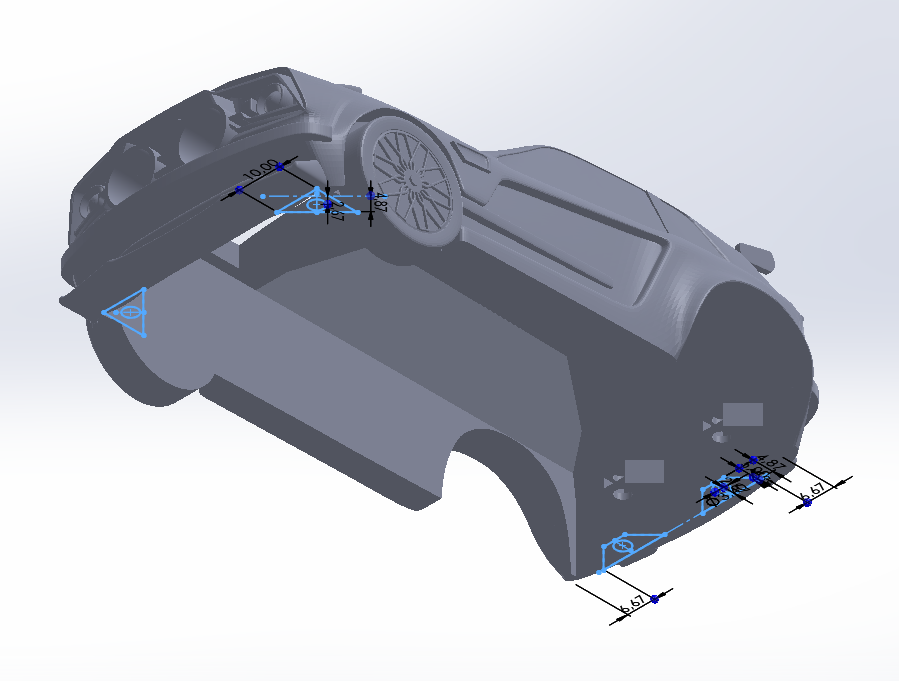
\includegraphics[width=0.4\textwidth]{images/solidworks/solidworks2.png}
    \caption{Conception 3D des emplacements vis}
    \label{fig:Conception 3D emplacements vis}
\end{figure}

\subsection{Taille de notre robot}
La troisième difficulté est lié à la deuxième, la limite de temps d'impression et le modèle 3D compact nous a poussé à devoir optimiser l'espace occupé par les composants, en utilisant des câbles femelle-femelle, ressoudant les branches de l'I2C, raccourcir nos cables etc.

Pour finir nous avons trouver une solution à chacun de nos problèmes grâce aux idées de chacun et des conseils des encadrants de TP, ce qui nous a permis d'arriver à un résultat convenable et fonctionnel.

\newpage